\documentclass{report}
\usepackage{graphicx}
\graphicspath{ {./screenshots/} }
\usepackage{titlesec}
\usepackage{float}
\usepackage{amsmath}
\usepackage{amssymb}
\usepackage{listings}

\titleformat{\chapter}[display]
  {\normalfont\bfseries}{}{0pt}{\Large}
\titlespacing*{\chapter}{0pt}{-100pt}{25pt}


\begin{document}

\begin{center}
    \large Zusammenfassung
\end{center}

\begin{center}
    \Large \textit{Maschinelles Lernen}\\
    \vspace*{.5em}
    \normalsize \textit{WS 19/20}\\
    \vspace*{45em}
    \large \today
\end{center}

\newpage

\chapter{Grundlagen}
\vspace*{-1.25em}
\section{Lineare Algebra}
\subsection{Skalarprodukt}
- Vektoren $x, y \in \mathbb{R}^n$: $x\circ y = \sum_{i=1}^n x_i\cdot y_i = x^Ty$\\
- $\begin{bmatrix}1\\2\end{bmatrix}\circ \begin{bmatrix}3\\4\end{bmatrix} = 1\cdot 3 + 2\cdot 4 = 11$
\subsection{Vektornorm}
$f: \mathbb{R}^n\rightarrow \mathbb{R}$ mit\\
\vspace*{-1.5em}
\begin{itemize}
  \item $f(x) = 0 \Rightarrow x = 0$
  \item $f(x + y) \leq f(x) + f(y)$ (\textit{Dreiecksgleichung})
  \item $f(\alpha x) = |\alpha|f(x)$
\end{itemize}
- $L_1$-Norm: $||x||_1 = \sum_i|x_i|$\\
- $L_2$-Norm: $||x||_2 = \sqrt{\sum_i x_i^2}$ (\textit{euklidische Norm})
\subsection{Matrizen}
- \textit{m} Zeilen und \textit{n Spalten}
A = $\begin{bmatrix}A_{11} & ... & A_{1n}\\A_{m1} & ... & A_{mn} \end{bmatrix}$,
$\begin{bmatrix}1 & 2\\3 & 4\\5 & 6\end{bmatrix}^T = \begin{bmatrix}1 & 3 & 5\\2 & 4 & 6\end{bmatrix}$\\
- $\begin{bmatrix}a & b & c\\d & e & f\end{bmatrix}\cdot \begin{bmatrix}g & h\\i & j\\k & l\end{bmatrix}$
= $\begin{bmatrix}ag + bi + ck & ah + bj + cl\\dg + ei + fk & dh + ej + fl\end{bmatrix}$,
$I = \begin{bmatrix}1 & 0 & 0\\0 & 1 & 0\\0 & 0 &1\end{bmatrix}$\\
- $A^{-1}A = I$ (Matrizen mit linear abhängigen Zeilen oder Spalten (niedriger Rang) sind nicht invertierbar)
\subsection{Hyperebene}
- x $\in$ $\mathbb{R}^d$ erfüllen Gleichung $w_0 + w_1x_1 + w2_x2 + ... + w_dx_d = 0$ ($w_0 + w^Tx = 0$)\\
- $d = 1$: Skalar ($w_0 + w_1x_1$), $d = 2$: Gerade ($w_0 + w_1x_1 + w_2x_2$), $d = 3$: Ebene\\
- Für einen Punkt $x$ entscheidet das Vorzeichen $sgn(w_0 + w^Tx)\in \{-1, 0, 1\}$ auf welcher Seite der Hyperebene er liegt (bzw. ob er auf ihr liegt)\\
\begin{center}
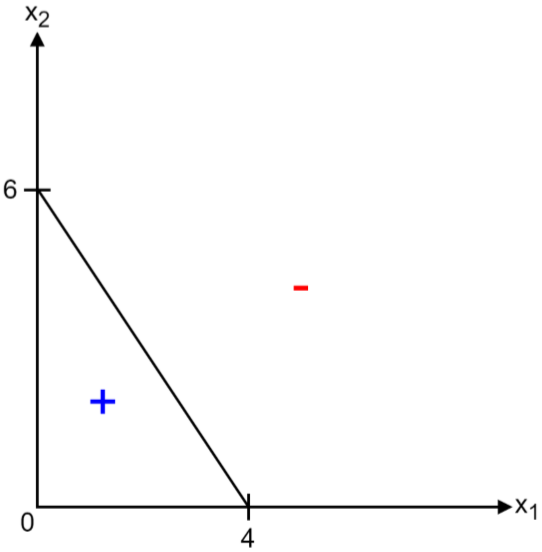
\includegraphics[scale=.2]{ml01_1} $1 - \frac{1}{4}x_1 - \frac{1}{6}x_2 = 0$
\end{center}

\section{Analysis}
\subsection{Kettenregel}
- Wenn $z$ von $y$ und $y$ von $x$ abhängt, dann gilt: $\frac{dz}{dx} = \frac{dz}{dy}\frac{dy}{dx}$\\
- $f(x) = g(h(x)) = \frac{1}{2}\cdot(x_1 - x_2)^2$ $\rightarrow$ $g(x) = \frac{1}{2}x^2$ und $h(x) = x_1 - x_2$\\
- $\frac{df}{dx_2} = \frac{dg}{dh}\frac{dh}{d_x2} = h(x)(-1) = -(x_1 - x_2) = x_2 - x_1$
\subsection{Partielle Ableitung}
$f(x) = 2x_1^3 - 5x_2^2 + 3$, $\frac{df}{dx_1} = 6x_1^2$, $\frac{df}{dx_2} = -10x_2$
\subsection{Gradient}
$\nabla f = \begin{bmatrix}\frac{df}{dx_1}\\ . \\. \\.\\\frac{df}{dx_n}\end{bmatrix}$, $f(x) = 2x_1^3 - 5x_2^2 + 3, \nabla f = \begin{bmatrix}6x_1^2\\-10x_2\end{bmatrix}$

\section{Was ist maschinelles Lernen}
\subsection{Paradigmenwechsel}
Es ist schwierig, den entsprechenden Programmcode manuell zu schreiben, daher wird ein anderes Paradigma verwendet:
\begin{center}
  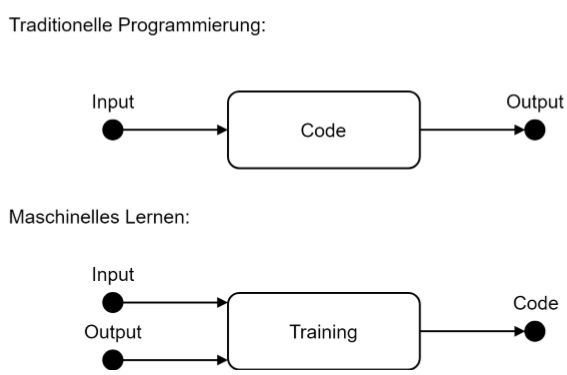
\includegraphics[scale=.4]{ml01_2}
\end{center}
Drei verschiedene Lernmethoden
\begin{itemize}
  \item Überwachtes Lernen (\textit{Supervised Learning})
  \item Unüberwachtes Lernen (\textit{Unsupervised Learning})
  \item Bestärkendes Lernen (\textit{Reinforcement Learning})
\end{itemize}

\section{Überwachtes Lernen}
- Ziel: finden einer Funktion $f: X \rightarrow Y$ wobei $X$ auch \textit{Features / Prädiktoren} und $Y$ auch \textit{Responses} genannt werden\\
- $X$ = $\mathbb{R}^d$ (\textit{d}-dimensionaler Vektorraum) mit $d\in \mathbb{N}$\\
- Eine perfekte Abbildung ist nicht möglich, es treten \textit{reduzierbare} Fehler (z.B. durch eine bessere Funktion $f$) und \textit{nicht reduzierbare} Fehler (z.B. Messfehler in Eingabedaten) auf\\
\vspace*{-1.5em}
\begin{itemize}
  \item \textit{Vorhersage:} $y = f(x)$ optimieren wobei $f$ auch \textit{Blackbox} sein kann
  \item \textit{Inferenz:} Interpretierbarkeit von $f$ steht im Vordergrund (Welche Prädiktoren sind für welche Response verwantwortlich)
  \item \textit{Parametrische} Methoden: Annahme einer parametrisierten Struktur von $f$ dessen Parameter mit Hilfe von Daten bestimmt werden
  \item \textit{Nicht-parametrische} Methoden: Keine Annahme einer Struktur von $f$ sondern möglichst direkte Definition mit Hilfe von Daten
\end{itemize}
- Menge $X$ und $Y$ bekannt, genaue Abbildung $f$ kann aber nur anhand von Beispielen $D = \{(x^i, y^i) | x^i \in X, y^i \in Y, 1 \leq i \leq n\}$ (\textit{Trainingsdatensatz} bzw. \textit{gelabelte} Daten) erahnt werden\\

\subsection{Beispiel Klassifikation}
- Wenn $Y$ diskrete Menge $\{C_1, ..., C_k\}$ für $k \in \mathbb{N}$ dann handelt es sich um ein \textit{Klassifikationsproblem}, $C_1, ..., C_k$ sind dann \textit{Klassen / Kategorien}\\
- $|Y| = 2$ (\textit{Binäre} Klassifikation) mit $f : \mathbb{R} \rightarrow \{$angenehm, unangenehm$\}$ (Temperaturklassifikation)\\
- $|Y| = 5$ (\textit{Mehrklassen}-Klassifikation) mit $f : \mathbb{R} \rightarrow \{$frostig, kalt, angenehm, warm, heiß$\}$

\subsection{Beispiel Regression}
- Wenn $Y$ kontinuierliche Menge, d.h. $Y \subseteq \mathbb{R}$, dann handelt es sich um ein \textit{Regressionsproblem}\\
- Interesse an \textit{quantitativen} Aussagen\\
\begin{center}
  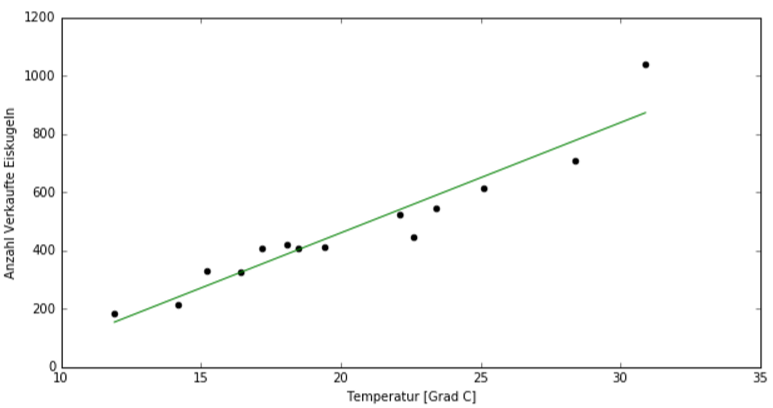
\includegraphics[scale=.4]{ml01_3}
\end{center}
- Ausgabemenge $Y$ kann auch mehrdimensional sein (z.B. $\{$gut, schlecht$\}\times \{$günstig, normal, teuer$\}$)

\section{Unüberwachtes Lernen}
- Mehrwert erhalten ohne Zuhilfenahme von gelabelten Daten\\
- Man geht von Menge an Daten $D = \{x^i|x^i \in X, 1 \leq i \leq n\}$ aus und versucht mehr über Beschaffenheit von $X$ herauszufinden\\
- z.B. \textit{Verteilung} von $X$ bei Sprachmodellen, \textit{Dimensionsreduktion} zur Verbesserung von überwachten Lernverfahren

\section{Datenvisualisierung}
\begin{figure}[H]
  \centering
  \begin{minipage}[b]{0.4\textwidth}
    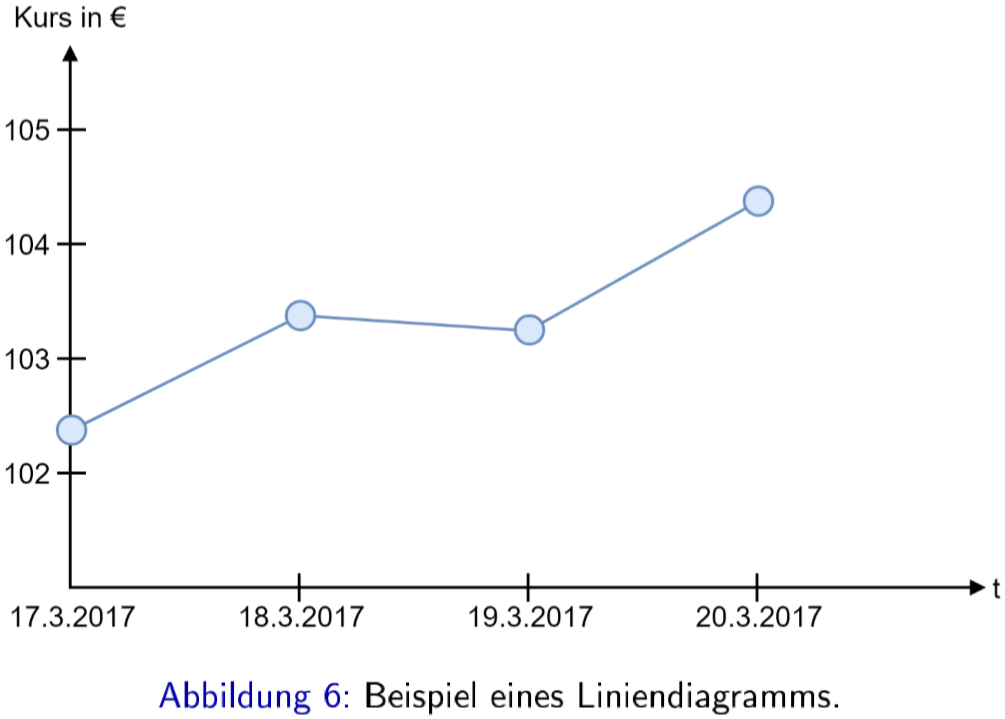
\includegraphics[scale=.25]{ml01_4}
  \end{minipage}
  \hfill
  \begin{minipage}[b]{0.4\textwidth}
    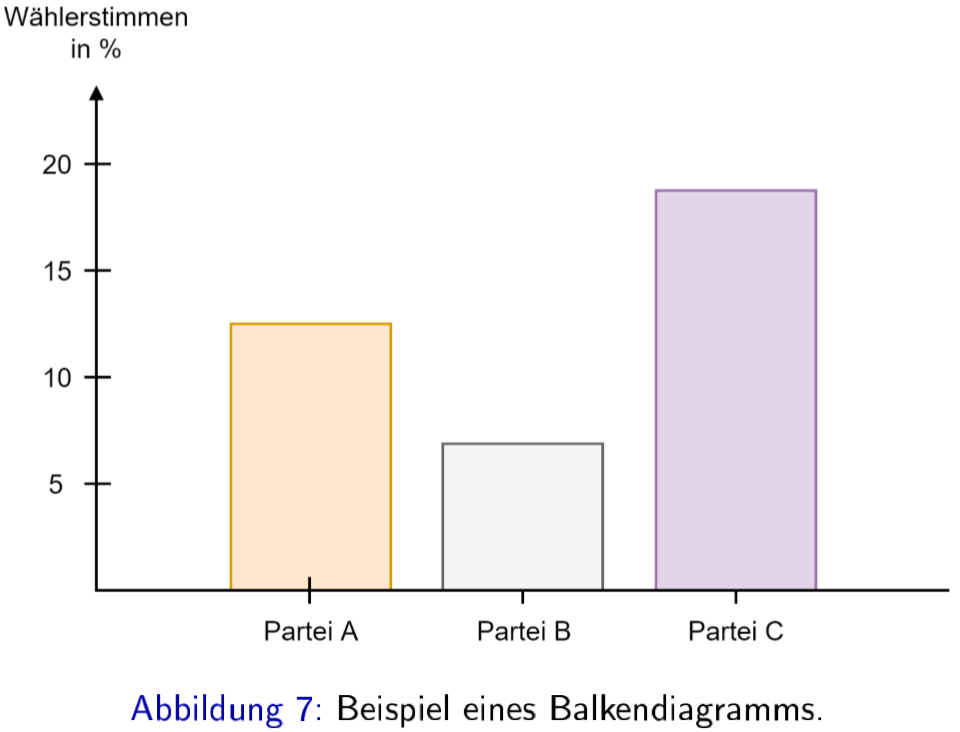
\includegraphics[scale=.25]{ml01_5}
  \end{minipage}
\end{figure}
\begin{figure}[H]
  \centering
  \begin{minipage}[b]{0.4\textwidth}
    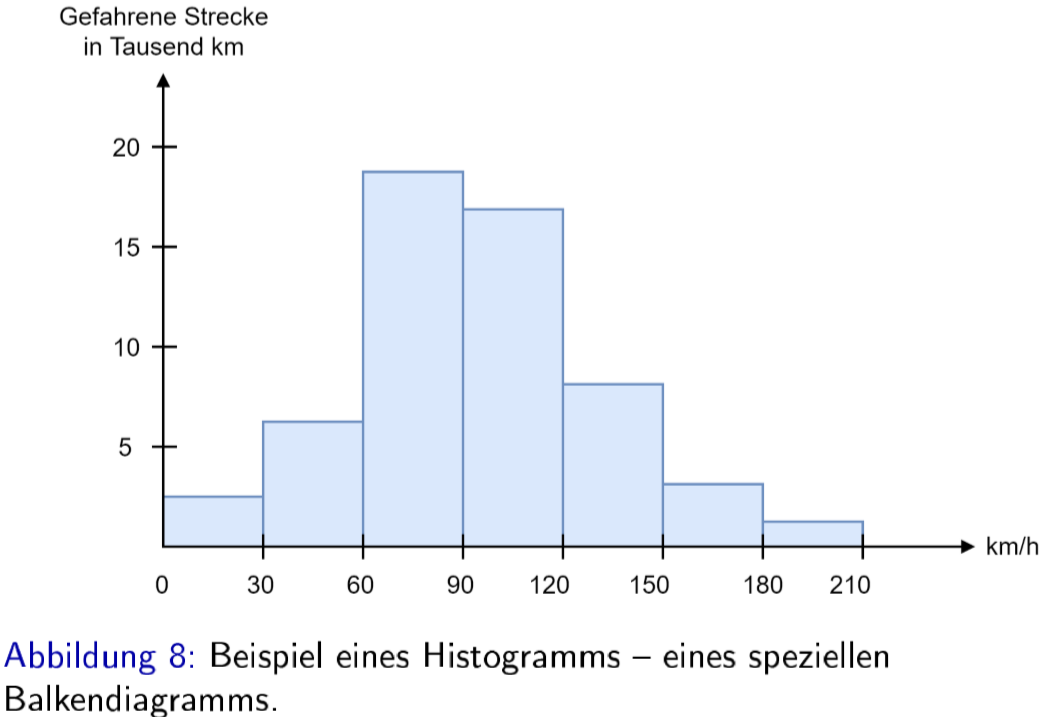
\includegraphics[scale=.25]{ml01_6}
  \end{minipage}
  \hfill
  \begin{minipage}[b]{0.4\textwidth}
    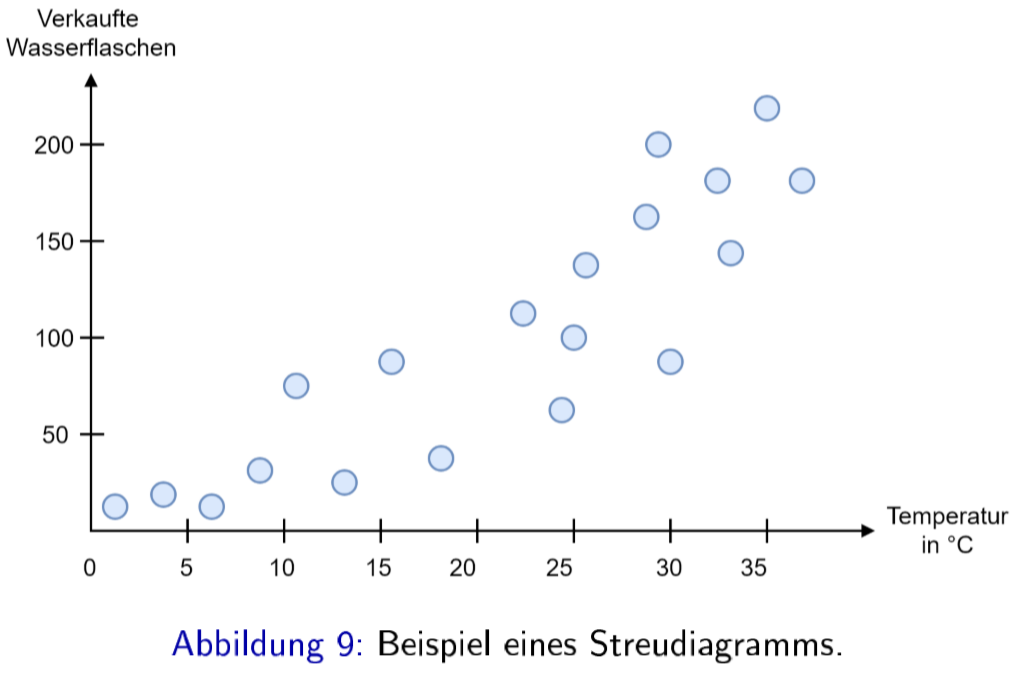
\includegraphics[scale=.25]{ml01_7}
  \end{minipage}
\end{figure}

\section{Datenvorverarbeitung}
Bevor ein Modell erstellt und trainiert werden kann, müssen Daten durch\\
\vspace*{-1.5em}
\begin{itemize}
  \item \textit{Auswahl}: Nur für den Anwendungsfall relevante Daten verwenden
  \item \textit{Aufbereitung}
  \subitem Dateiformat (Tabellen, BigData)
  \subitem Bereinigung von unvollständigen oder ungültigen Daten
  \subitem Repräsentative Auswahl bei langer Laufzeit / großem Speicheraufwand
  \item \textit{Transformation}
  \subitem Features in geeigneten Wertebereich bringen ([0, 1])
  \subitem Zerlegen in sinnvolle Features
  \subitem Aggregation mehrerer Features
\end{itemize}

\chapter{Lineare Regression}
\section{Lineare Regression im Eindimensionalen}
- $f : \mathbb{R} \rightarrow \mathbb{R}$ mit $f_w(x) = w_1x + w_0$\\
- $w = (w_0, w_1)^T \in \mathbb{R}^2$ sind die \textit{Parameter} des Modells
\begin{center}
  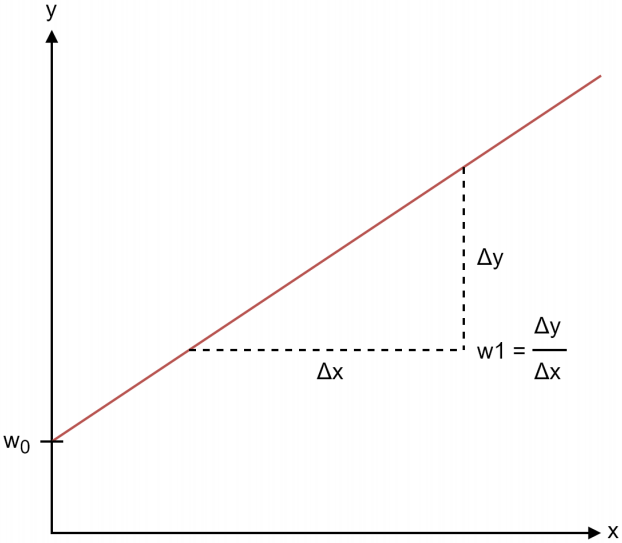
\includegraphics[scale=0.275]{ml02_1}
\end{center}
- Wie mit Daten $D = \{(x^i, y^i) \in \mathbb{R}^2 | 1 \leq i \leq n\}$ die \textit{besten} Parameter von $f$ bestimmen?\\
\subsection{Lösungsverfahren}
- Quadratischen Fehler (\textit{Residual Sum of Squares}) mit\\
$RSS(w) = \sum_{i=1}^n(y^i - f_w(x^i))^2$ bestimmen
\begin{center}
  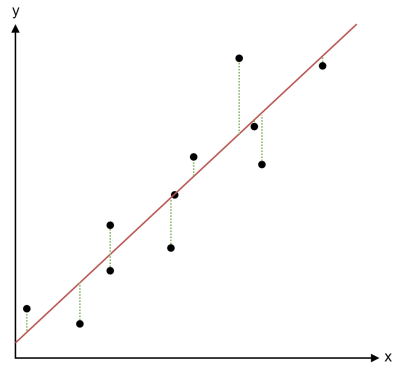
\includegraphics[scale=0.35]{ml02_2}
\end{center}
- Zur besseren Vergleichbarkeit verwendet man oft die normalisierte Variante\\
\textit{Mean Squared Error}: $MSE(w) = \frac{1}{n}\cdot RSS(w)$ (n = Anzahl Trainingsdaten)\\
- Die beste Funktion durch Minimierung des Fehlers finden
$\Rightarrow w^* =$ arg min $E(w) =$ arg min $\frac{1}{2}\cdot \sum_{i=1}^n(y^i - f_w(x^i))^2$\\
\vspace*{-1.25em}
\begin{itemize}
  \item Ableitung von $E(w)$ gleich Null setzen und Gleichungssystem lösen
  \item $\nabla E(w) = \begin{bmatrix}\frac{dE(w)}{dw_0}\\\frac{dE(w)}{dw_1}\end{bmatrix} = 0$
  \subitem $\frac{dE(w)}{dw_0} = -\sum_{i=1}^ny^i + w_1\cdot \sum_{i=1}^nx^i + n\cdot w_0$
  \subitem $\frac{dE(w)}{dw_1} = -\sum_{i=1}^nx^iy^i + w_1\cdot \sum_{i=1}^nx^ix^i + w_0\cdot \sum_{i=1}^nx^i$
  \item Gleichungssystem mit zwei Gleichungen und zwei Unbekannten lösbar, aber numerisch ungenau bei großen Matrizen 
\end{itemize}

\subsection{Gradientenabstiegsverfahren}

\begin{center}
  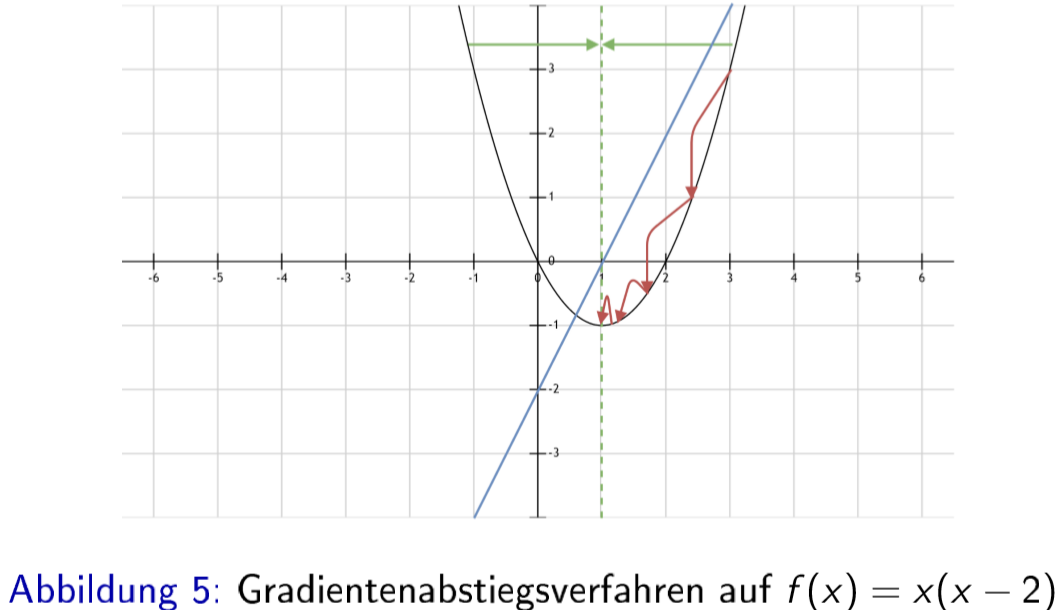
\includegraphics[scale=.25]{ml02_3}
\end{center}
- Iterativ einem Bruchteil der negativen Ableitung: $-\eta f'(x) = \eta\cdot (2 - 2x)$ folgen\\
- \textit{Lernrate} $\eta$ hat direkten Einfluss auf Konvergenz (zu klein $\Rightarrow$ viele Schritte, zu groß $\Rightarrow$ Oszillation)\\
\begin{lstlisting}
  w0 = 0, w1 = 0
  for (x, y) in D
    dw0 += -y + w1*x + w0
    dw1 += -xy + w1*x*x + w0*x
  end for
  w0 += -eta*dw0
  w1 += -eta*dw1
\end{lstlisting}

\section{Mehrdimensionale Lineare Regression}
- $X = \mathbb{R}^d$ und $f: \mathbb{R}^d \rightarrow \mathbb{R}$ sowie $f_w(x) = \sum_{i=1}^dw_ix_i + w_0$\\
mit Parametern $w = (w_0, w_1, ..., w_d)^T \in \mathbb{R}^{d + 1}$
- Kompaktere Schreibweise mit $x_0 = 1$: $f_w(x) = \sum_{i = 1}^dw_ix_i + w_0 = w^Tx$\\
\begin{center}
  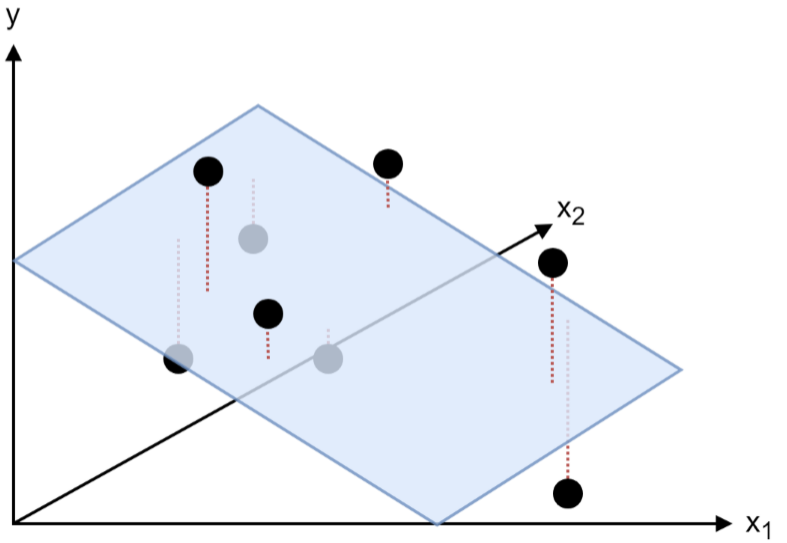
\includegraphics[scale=.25]{ml02_4}
\end{center}
- Im Mehrdimensionalen wird eine Hyperebene, im dreidimensionalen eine Ebene, im Raum so positioniert, dass der Abstand zu den Datenpunkten minimiert wird\\
- Angepasste Fehlermetrik $E(w) = \frac{1}{2}\cdot \sum_{i=1}^n(y^i - f(x^i))^2$
mit $\nabla E(w) = \begin{bmatrix}\frac{dE(w)}{dw_0}\\\frac{dE(w)}{dw_1}\\...\\\frac{dE(w)}{dw_d}\end{bmatrix}$\\
\begin{lstlisting}
  dw = 0
  for (x, y) in D
    dw += -(y - f(x) * gradF(x))
  end for
  w += -eta*dw
\end{lstlisting}
wobei gradF(x) = $\nabla f(x) = \begin{bmatrix}1\\x_1\\...\\x_d\end{bmatrix}$\\
\begin{center}
  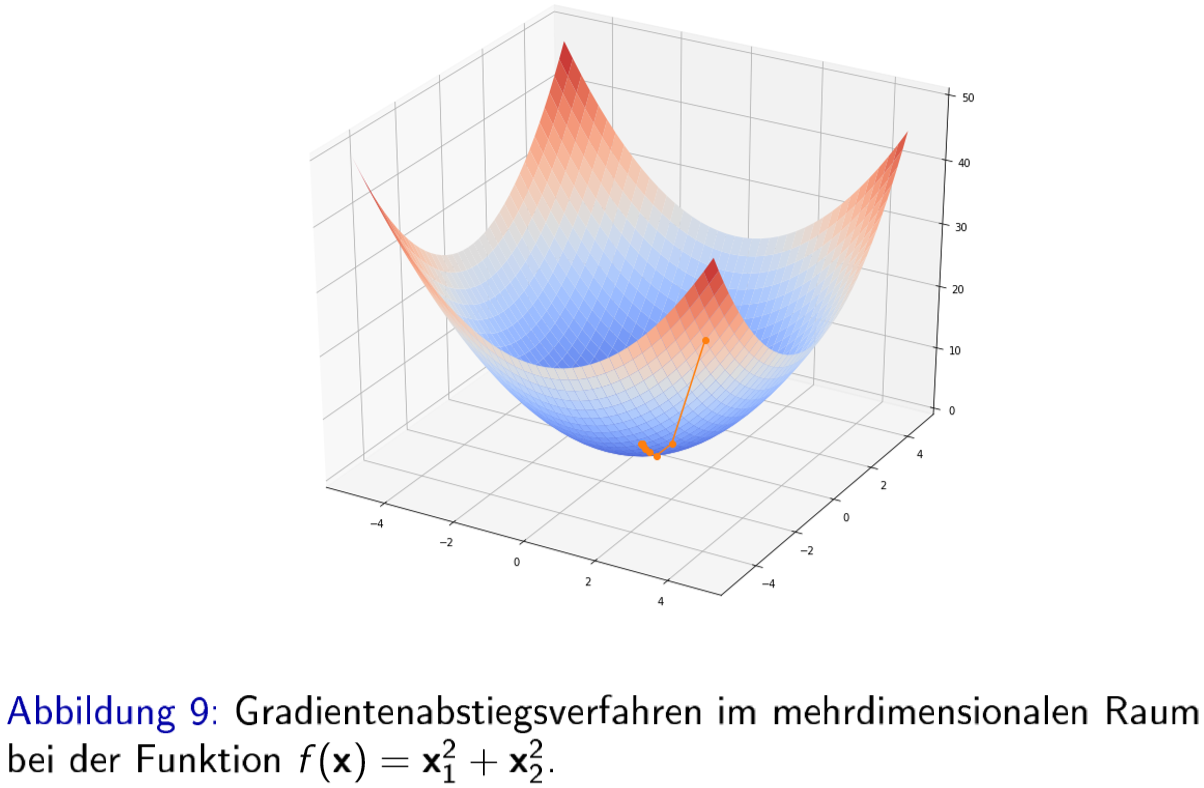
\includegraphics[scale=.25]{ml02_5}
\end{center}

\section{Genauigkeit}
- Wie gut ist das durch das Gradientenabstiegsverfahren gefundene Modell?\\
$\Rightarrow$ Quadratischer Fehler \textit{RSS} oder mittlerer quadratischer Fehler \textit{MSE}\\
- Letzterer ist unabhängig von der Anzahl an Trainingsdaten allerdings gibt es keine allgemein gültige Skala da diese vom Wertebereich der y-Werte abhängt

\subsection{$R^2$ Statistik}
- Definiert über den quadratischen Gesamtfehler $TSS = \sum_{i=1}^n(y^i - \bar{y})^2$\\
- $\bar{y} = \frac{1}{n}\cdot \sum_{i=1}^ny^i$ $\Rightarrow$ $R^2(w) = \frac{TSS - RSS(w)}{TSS} = 1 - \frac{RSS(w)}{TSS}$\\
- \textit{TSS} misst die komplette Varianz in den Ausgabedaten $y^i$\\
- $TSS - RSS(w)$ misst die durch das Modell mit Parametern $w$ erklärte Varianz\\
- $R^2$ misst die komplette Varianz des Modells und ist $\in [0, 1]$\\
\vspace*{-1.25em}
\begin{itemize}
  \item $R^2$ nahe 1 zeugt von einem passenden Model das die Daten gut erklärt
  \item $R^2$ nahe 0 bedeutet, dass das Modell die Daten schlecht erklärt
\end{itemize}
- $R^2$ ist unabhängig von Anzahl an Trainingsdaten \textit{UND} dem Wertebereich\\
- Allgemeine Aussage ab welchem $R^2$-Wert das Modell \textit{gut} ist, ist nicht möglich. Hängt vom Anwendungsfall (Medizin / Physik) ab

\section{Interpretierbarkeit}

\end{document}